\let\negmedspace\undefined
\let\negthickspace\undefined
\documentclass[journal]{IEEEtran}
\usepackage[a5paper, margin=10mm, onecolumn]{geometry}
%\usepackage{lmodern} % Ensure lmodern is loaded for pdflatex
\usepackage{tfrupee} % Include tfrupee package

\setlength{\headheight}{1cm} % Set the height of the header box
\setlength{\headsep}{0mm}  % Set the distance between the header box and the top of the text

\usepackage{gvv-book}
\usepackage{gvv}
\usepackage{cite}
\usepackage{amsmath,amssymb,amsfonts,amsthm}
\usepackage{algorithmic}
\usepackage{graphicx}
\usepackage{textcomp}
\usepackage{xcolor}
\usepackage{txfonts}
\usepackage{listings}
\usepackage{enumitem}
\usepackage{mathtools}
\usepackage{gensymb}
\usepackage{comment}
\usepackage[breaklinks=true]{hyperref}
\usepackage{tkz-euclide} 
\usepackage{listings}
% \usepackage{gvv}                                        
\def\inputGnumericTable{}                                 
\usepackage[latin1]{inputenc}                                
\usepackage{color}                                            
\usepackage{array}                                            
\usepackage{longtable}                                       
\usepackage{calc}                                             
\usepackage{multirow}                                         
\usepackage{hhline}                                           
\usepackage{ifthen}                                           
\usepackage{lscape}
\begin{document}

\bibliographystyle{IEEEtran}
\vspace{3cm}

\title{9.4.5}
\author{EE24BTECH11021 - Eshan Ray}

% \maketitle
% \newpage
% \bigskip
{\let\newpage\relax\maketitle}

\renewcommand{\thefigure}{\theenumi}
\renewcommand{\thetable}{\theenumi}
\setlength{\intextsep}{10pt} % Space between text and floats

\textbf{Question:}\\
For the Differential Equation $\brak{e^{-x} + e^{x}}dy-\brak{e^x-e^{-x}}dx=0$, find  a general  solution of the differential equation.

\solution{
Solving the given D.E. , we get,
\begin{align}
    \brak{e^{-x} + e^{x}}dy-\brak{e^x-e^{-x}}dx &= 0\\
    \implies    \frac{dy}{dx} &= \frac{e^{x}-e^{-x}}{e^{-x}+e^x}\\
    \implies    \frac{dy}{dx} &= \frac{e^{2x}-1}{e^{2x}+1}    
\end{align}
Substituting, $t = e^{2x}$, we get,
\begin{align}
    \implies    dt &= 2e^{2x}dx\\
    \implies    dx &= \frac{dt}{2t}\\
    \implies    \frac{dy}{\brak{\frac{dt}{2t}}} &= \frac{t-1}{t+1}\\
    \implies    \frac{dy}{dt} &= \frac{t-1}{2t\brak{t+1}}\\
    \implies    \frac{dy}{dt} &= \frac{1}{2}\brak{\frac{1}{\brak{t+1}} -\frac{1}{t\brak{t+1}}}\\
    \implies    dy &= \frac{1}{2}\brak{\frac{2}{t+1}-\frac{1}{t}}dt\\
\end{align}
Integrating both sides, we get,
\begin{align}
    \implies    \int dy &= \int \frac{dt}{t+1} - \int \frac{dt}{2t}\\
    \implies    y &= \ln{\abs{t+1}} - \frac{1}{2}\ln{\abs{t}} +C\\
\end{align}
substituting, $t = e^{2x}$
\begin{align}
    \implies    y &= \ln{\abs{e^{2x}+1}}- \frac{1}{2}\ln{\abs{e^{2x}}} +C\\
    \implies    y &= \ln{\brak{e^{2x}+1}} - x +C
\end{align}
\textbf{Computational Solution:}\\
Using Trapezoidal rule, we get,\\
\begin{align}
   f\brak{x} &= \frac{dy}{dx}\\
   \int_{x_0}^{x_n} f\brak{x} &\approx \frac{h}{2}\brak{\brak{f\brak{x_0}+f\brak{x_1}}+\brak{f\brak{x_1}+f\brak{x_2}}+\dots\brak{f\brak{x_{n-1}}+f\brak{n}}}\\
   \int_{x_0}^{x_n}f\brak{x} &\approx \frac{h}{2}\brak{f\brak{x_0}+f\brak{x_n}+2\sum_{i=1}^{n-1}f\brak{x_i}}\\
\end{align}
Using Trapezoid rule for discretizing the steps , we get,
\begin{align}
    y_{n+1} - y_n &= \frac{h}{2}\brak{f\brak{x_n}+f\brak{x_{n+1}}}\\
\end{align}
By the classical definition of derivative we know that $f\brak{x_{n+1}} = f\brak{x_n} + hf\prime\brak{x_n}$
\begin{align}
    y_{n+1} - y_{n} &= \frac{h}{2}\brak{f\brak{x_n} + f\brak{x_n} + hf\prime\brak{x_n}}\\
    y_{n+1} &= y_n + hf\brak{x_n} + \frac{h^2}{2}f\prime\brak{x_n}
\end{align}
The difference equation,
\begin{align}
    y_{n+1} &= y_n + h\frac{e^{2x_n}-1}{e^{2x_n}+1} + \frac{h^2}{2}\frac{4e^{2x_n}}{\brak{e^{2x_n}+1}^2}\\
    x_{n+1} &= x_n + h
\end{align}

The initial conditions for the plotting of graph are as follows:-
\begin{align}
    x_0 &= -5\\
    y_0 &= 5\\
    h &= 0.01\\
    C &= 0
\end{align}

\begin{figure}[h]
    \centering
    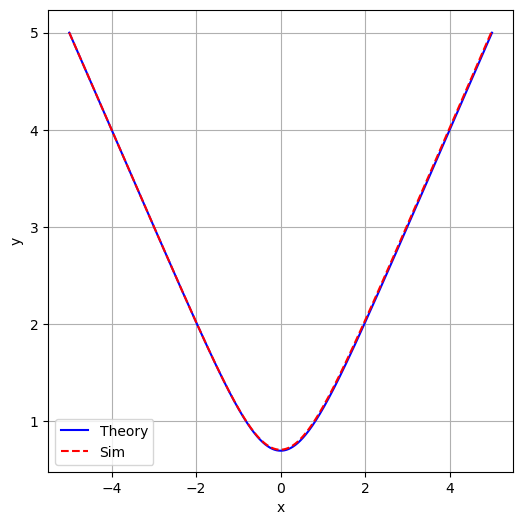
\includegraphics[width=\columnwidth]{plots/plot.png}
    \caption{Plot of the differential equation when $h=0.01$}
    \label{fig:Plot1}
    \end{figure}

\end{document}
